% 独立编译：latexmk -cd -xelatex -interaction=nonstopmode -file-line-error 第一部分_网格与位移求解.tex
% 依赖同目录assets/；无参考文献数据库；数值表由../prepare_stage1.py生成。
\documentclass[UTF8,a4paper,fontset=fandol,10pt]{ctexart}
\usepackage{amsmath,amssymb,bm,upgreek}
\newcommand{\dd}{\mathop{}\!\mathrm{d}}
\newcommand{\ee}{\mathrm{e}}
\newcommand{\ii}{\mathrm{i}}
\usepackage{booktabs,array,longtable,graphicx,caption,subcaption,float,tikz}
\usepackage{xcolor,listings,siunitx}
\definecolor{ink}{HTML}{183247}
\definecolor{accent}{HTML}{B55537}
\usepackage[colorlinks=true,allcolors=ink]{hyperref}
\usepackage{cleveref}
\crefname{figure}{图}{图}\crefname{table}{表}{表}\crefname{equation}{式}{式}
\crefformat{section}{第#2#1#3节}
\usepackage{geometry,fancyhdr}
\geometry{left=24mm,right=24mm,top=23mm,bottom=23mm}
\pagestyle{fancy}\fancyhf{}
\fancyhead[L]{\small 二维悬臂梁有限元计算}
\fancyhead[R]{\small 计算与结果分析}
\fancyfoot[C]{\small\thepage}
\setlength{\headheight}{14pt}
\setlength{\parskip}{4pt}
\setlength{\emergencystretch}{2em}
\ctexset{section={format=\large\bfseries\color{ink}},subsection={format=\normalsize\bfseries\color{ink}}}
\captionsetup{font=small,labelfont=bf}
\graphicspath{{assets/}}
\newcommand{\code}[1]{\texttt{\detokenize{#1}}}
\lstset{language=Python,basicstyle=\ttfamily\small,breaklines=true,
 backgroundcolor=\color{ink!4},frame=single,rulecolor=\color{ink!20},showstringspaces=false}
\title{\vspace{-1.2em}\color{ink}\LARGE 二维悬臂梁：从单元刚度到节点位移\\[.4em]
\large 三套网格：线弹性与J2弹塑性分析}
\author{\small 求解代码见 GitHub：\href{https://github.com/RicardoMFu/cantilever-fem}{\texttt{RicardoMFu/cantilever-fem}}}\date{2026年11月1日}
\begin{document}
\maketitle\vspace{-2em}

\section{模型与参数}
计算域为$0\leq x\leq20\,\mathrm m$、$0\leq y\leq1\,\mathrm m$。
材料取$E=210\,\mathrm{GPa}$、$\nu=0.30$，采用\textbf{小应变、线弹性、平面应变}模型。
左端全部节点满足$u=v=0$；右端全部节点满足$v=-0.1\,\mathrm m$，水平位移$u$保持自由。
上下表面无外加面力，忽略体力。以$u,v$分别表示水平和竖向位移。

\begin{figure}[H]\centering
\begin{tikzpicture}[x=0.5cm,y=1cm,>=stealth]
\fill[ink!6] (0,0) rectangle (20,1);
\draw[ink] (0,0) rectangle (20,1);
\draw[ink,line width=1.4pt] (0,-.2)--(0,1.2);
\foreach \q in {-.1,.15,.4,.65,.9,1.15}{\draw[ink](-.4,\q-.15)--(0,\q);}
\draw[ink,dashed] (0,.5)--(20,.5);
\draw[accent,->,thick] (20,1.5)--(20,-.65);
\node[anchor=west] at (20.3,.5) {$v=-0.1\,\mathrm m$};
\node[anchor=west] at (20.3,0) {$u$自由};
\draw[<->] (0,-.65)--(20,-.65) node[midway,below] {$L=20\,\mathrm m$};
\draw[<->] (-1.4,0)--(-1.4,1) node[midway,left] {$h=1\,\mathrm m$};
\node[anchor=south] at (10,1.25) {线弹性、平面应变；$E=210\,\mathrm{GPa}$，$\nu=0.30$};
\node[anchor=north] at (3,-1.15) {左端：$u=v=0$};
\node[anchor=north] at (14,-1.15) {上下表面：无外加面力};
\end{tikzpicture}
\caption{几何、材料与边界条件示意。箭头表示规定的位移方向，图形比例作显示调整。}
\end{figure}


原题只给厚度符号$b$，未指定数值，本计算明确取$b=1\,\mathrm m$。
对本题均匀厚度、纯位移加载的设置，$K$与反力均随$b$成正比，位移解不随$b$改变。
厚度约定需要保留在后续反力和能量结果中。

本文完成三套网格的位移求解、挠度比较、应力恢复和指定点应力分析。线弹性使用NumPy直接求解；弹塑性使用SciPy稀疏直接求解与Newton迭代。未使用有限元软件或高层有限元库。

\begin{table}[H]\centering
\caption{三套网格与方程规模}\label{tab:counts}
\begin{tabular}{rrrrrr}\toprule 网格 & 单元数 & 节点数 & 总自由度 & 已知位移数 & 待求位移数\\\midrule
$8\times2$ & 16 & 27 & 54 & 9 & 45 \\
$16\times4$ & 64 & 85 & 170 & 15 & 155 \\
$32\times8$ & 256 & 297 & 594 & 27 & 567 \\
\bottomrule\end{tabular}

\end{table}

\subsection{节点与自由度编号}
令长度方向有$n_x$个单元，高度方向有$n_y$个单元。
节点先沿底边从左到右编号，再逐行向上；单元采用同样顺序。
用从零开始的行列指标$i,j$表示节点位置，则
\begin{equation}
 n(i,j)=j(n_x+1)+i+1,\qquad
 x_i=\frac{20i}{n_x},\quad y_j=\frac{j}{n_y}.
\end{equation}
节点$n$的全局位移编号是$g_u=2n-1$、$g_v=2n$。
局部节点统一按\textbf{左下、右下、右上、左上}逆时针排列。
对单元左下角指标$(i,j)$，单元号$e=jn_x+i+1$，有
\begin{equation}
 \mathrm{IEN}(:,e)=
 \begin{pmatrix}n(i,j)\\n(i,j)+1\\n(i,j)+n_x+2\\n(i,j)+n_x+1\end{pmatrix}.
\end{equation}
\textbf{IEN记录节点连接；ID记录自由方程编号。}本文ID对自由位移按全局顺序编为$1,2,\ldots,n_f$，
对已知位移标记为0。\textbf{ID为0表示位移已知，不代表该位移数值为0}；右端$v=-0.1\,\mathrm m$也标记为0。
完整ID与IEN数值见附录。

ID完整数组有$2\times n_n$项，IEN完整数组有$4\times n_e$项，
其中$n_n$和$n_e$分别是节点数与单元数。
IEN按单元号读取四个全局节点；ID按节点号及位移方向读取自由方程编号。附录逐条列出对应关系。


\section{单元矩阵}
四节点单元使用双线性形函数：
\begin{equation}
\begin{aligned}
N_1&=\tfrac14(1-\xi)(1-\eta),&N_2&=\tfrac14(1+\xi)(1-\eta),\\
N_3&=\tfrac14(1+\xi)(1+\eta),&N_4&=\tfrac14(1-\xi)(1+\eta).
\end{aligned}
\end{equation}
同一组形函数用于插值坐标和位移：$x=\sum_aN_ax_a$、$y=\sum_aN_ay_a$，
$u=\sum_aN_au_a$、$v=\sum_aN_av_a$。
标准坐标只用于方便积分，并没有增加物理位移未知量。

\subsection{应变矩阵}
采用下列雅可比矩阵约定：
\begin{equation}
J=\begin{pmatrix}x_{,\xi}&x_{,\eta}\\y_{,\xi}&y_{,\eta}\end{pmatrix},
\qquad
\begin{pmatrix}N_{a,x}\\N_{a,y}\end{pmatrix}
=J^{-\mathsf T}\begin{pmatrix}N_{a,\xi}\\N_{a,\eta}\end{pmatrix}.
\end{equation}
以工程剪应变$\gamma_{xy}=u_{,y}+v_{,x}$为第三分量，得到
\begin{equation}
\boldsymbol\varepsilon=\begin{pmatrix}\varepsilon_{xx}\\\varepsilon_{yy}\\\gamma_{xy}\end{pmatrix}
=B\mathbf d_e,\quad B=[B_1\ B_2\ B_3\ B_4],\quad
B_a=\begin{pmatrix}N_{a,x}&0\\0&N_{a,y}\\N_{a,y}&N_{a,x}\end{pmatrix}.
\end{equation}
这里$B$为$3\times8$，$\mathbf d_e=(u_1,v_1,u_2,v_2,u_3,v_3,u_4,v_4)^{\mathsf T}$。
平面应变本构矩阵为
\begin{equation}
D=\frac{E}{(1+\nu)(1-2\nu)}
\begin{pmatrix}1-\nu&\nu&0\\\nu&1-\nu&0\\0&0&(1-2\nu)/2\end{pmatrix}
=\begin{pmatrix}282.692308&121.153846&0\\121.153846&282.692308&0\\0&0&80.769231\end{pmatrix}\mathrm{GPa}.
\end{equation}

\subsection{单元刚度}
由虚功离散得到单元刚度，采用$2\times2$高斯完全积分：
\begin{equation}\label{eq:ke}
 K^{(e)}=b\int_{-1}^{1}\int_{-1}^{1}B^{\mathsf T}DB\det J\,\dd\xi\,\dd\eta
 \approx b\sum_{q=1}^{4}B_q^{\mathsf T}DB_q\det J_q.
\end{equation}
积分点为$(\pm1/\sqrt3,\pm1/\sqrt3)$的四种组合，两方向权重均为1。
每个点产生一个$8\times8$矩阵，四个矩阵逐项相加。

对$8\times2$网格第1单元，$\Delta x=2.5\,\mathrm m$、$\Delta y=0.5\,\mathrm m$，
$J=\operatorname{diag}(1.25,0.25)\,\mathrm m$，$\det J=0.3125\,\mathrm{m^2}$。
课堂中展开的第一个对角项和交叉项是
\begin{align}
(B^{\mathsf T}DB)_{11}&=D_{11}N_{1,x}^2+D_{33}N_{1,y}^2,\\
(B^{\mathsf T}DB)_{12}&=(D_{12}+D_{33})N_{1,x}N_{1,y}.
\end{align}
完成四点求和后，左上角小块为
\begin{equation}
K^{(1)}_{1:2,1:2}=b
\begin{pmatrix}153.461538&50.480769\\50.480769&476.538462\end{pmatrix}\mathrm{GPa}.
\end{equation}
乘入以米计的$b$后，刚度单位是$\mathrm{N/m}$。

\section{整体方程与位移}
\subsection{刚度组装}
单元内力满足$\mathbf f_e=K^{(e)}\mathbf d_e$。同一个全局节点可能连接多个单元，
它的总内力等于各相邻单元内力之和，因此对应刚度也必须相加：
\begin{equation}
 K_{g_i^{(e)},g_j^{(e)}}\mathrel{+}=K^{(e)}_{ij}.
\end{equation}
对粗网格，前两个单元的局部到全局自由度映射分别是
\[
\mathbf g^{(1)}=(1,2,3,4,21,22,19,20),\quad
\mathbf g^{(2)}=(3,4,5,6,23,24,21,22).
\]
例如全局节点2的水平自由度是3，它同时得到两个单元的贡献：
\[
 K_{33}=K^{(1)}_{33}+K^{(2)}_{11}
       =b\times306.923077\,\mathrm{GPa}.
\]
积分是在单元内部累加空间贡献；组装是在全局自由度位置累加相邻单元贡献。

\subsection{边界条件与求解}
用下标$f$表示位移待求的自由度，用$c$表示位移已知的自由度。本题无已知外加力，
自由位置的平衡条件为
\begin{equation}
 K_{ff}\mathbf d_f+K_{fc}\mathbf d_c=\mathbf0
 \quad\Longrightarrow\quad
 \boxed{K_{ff}\mathbf d_f=-K_{fc}\mathbf d_c.}
\end{equation}
粗网格的已知全局自由度和对应位移是
\[
c=(1,2,18,19,20,36,37,38,54),\quad
\mathbf d_c=(0,0,-0.1,0,0,-0.1,0,0,-0.1)^{\mathsf T}\,\mathrm m.
\]
所以$K_{ff}$为$45\times45$。右端水平自由度17、35、53保持未知，不能额外固定。
网格加密时只需按节点坐标寻找左右边界，不必手工修改这些编号。

\begin{lstlisting}
K[np.ix_(dofs, dofs)] += ke
Kff = K[np.ix_(free, free)]
rhs = -K[np.ix_(free, fixed)] @ d[fixed]
d[free] = np.linalg.solve(Kff, rhs)
reaction = K @ d
\end{lstlisting}
\code{np.ix_}提取行、列编号的全部组合；\code{free}与\code{fixed}分别存储两组全局下标。
\code{solve}调用LAPACK的一般线性系统直接解法，通过选主元LU分解及前后代入求解，
不显式计算矩阵逆。$\mathbf r=K\mathbf d$在自由位置应接近0，在已知位移位置给出支座或加载装置的反力。

\begin{table}[H]\centering
\caption{三套网格的实际求解结果，$b=1\,\mathrm m$}\label{tab:solutions}
\begin{tabular}{rrrr}\toprule 网格 & $v(10,0.5)$ / m & 右端竖向合反力 / kN & 自由位置相对残差\\\midrule
$8\times2$ & -0.03118569 & -2347.295 & $2.7e-13$ \\
$16\times4$ & -0.03115850 & -1131.167 & $2.5e-12$ \\
$32\times8$ & -0.03119089 & -824.732 & $1.1e-11$ \\
\bottomrule\end{tabular}

\end{table}
表中$v(10,0.5)$是一个点的位移，反力是右端所有受约束竖向自由度的力之和。
三套网格端部位移均为$-0.1\,\mathrm m$，但反力不同，对应等效端部刚度
$|R_y|/0.1$分别为$23.473$、$11.312$、$8.247\,\mathrm{MN/m}$。
这反映粗网格弯曲偏硬，而不是求解器没有解平衡。
自由位置相对残差按$\max_{i\in f}|(K\mathbf d)_i|/\max_{i\in c}|(K\mathbf d)_i|$计算，
只衡量离散方程的平衡程度，不能衡量与真实连续体解的误差。
刚度对称性按$e_K=\|K-K^{\mathsf T}\|_F/\|K\|_F$计算。
其中$\|A\|_F=\sqrt{\sum_i\sum_j A_{ij}^2}$，即全部矩阵项平方和的平方根。$e_K$比较同一网格的$K_{ij}$与$K_{ji}$，不比较不同网格的刚度。三套网格的$e_K$依次为$3.15\times10^{-17}$、$4.52\times10^{-17}$、$4.28\times10^{-17}$。
粗网格总矩阵的部分项（单位$\mathrm{GN/m}$）为
\[
K_{1:2,1:2}=\begin{pmatrix}153.461538&50.480769\\50.480769&476.538462\end{pmatrix},
\quad K_{12}=K_{21}=50.480769\,\mathrm{GN/m}.
\]


\section{网格编号图}
三图采用统一编号规则。左端深色线表示固定端，右端棕色线表示规定竖向位移的边界。

\begin{figure}[H]\centering
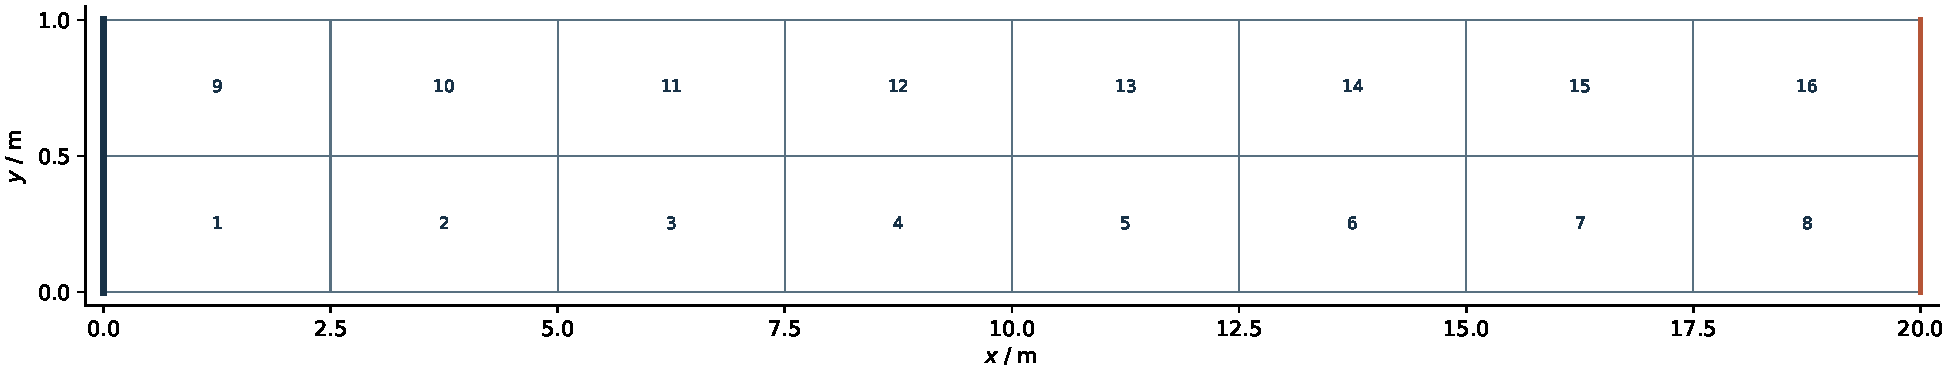
\includegraphics[width=\linewidth]{mesh_8x2.pdf}
\caption{$8\times2$网格，16个单元、27个节点。}
\end{figure}
\begin{figure}[H]\centering
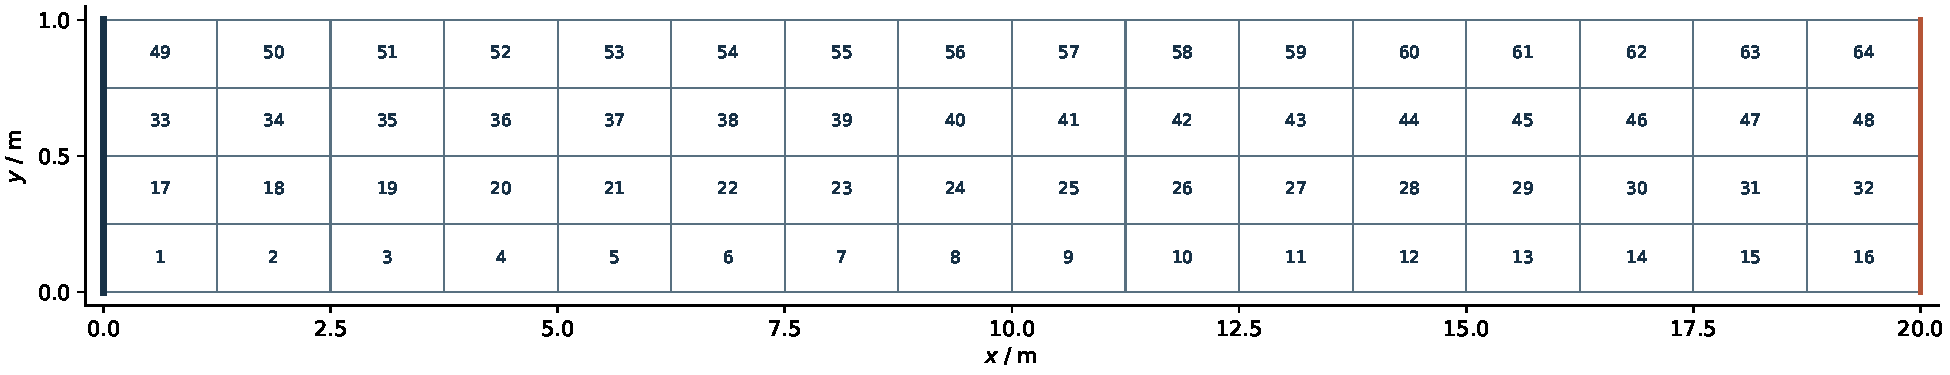
\includegraphics[width=\linewidth]{mesh_16x4.pdf}
\caption{$16\times4$网格，64个单元、85个节点。}
\end{figure}
\begin{figure}[H]\centering
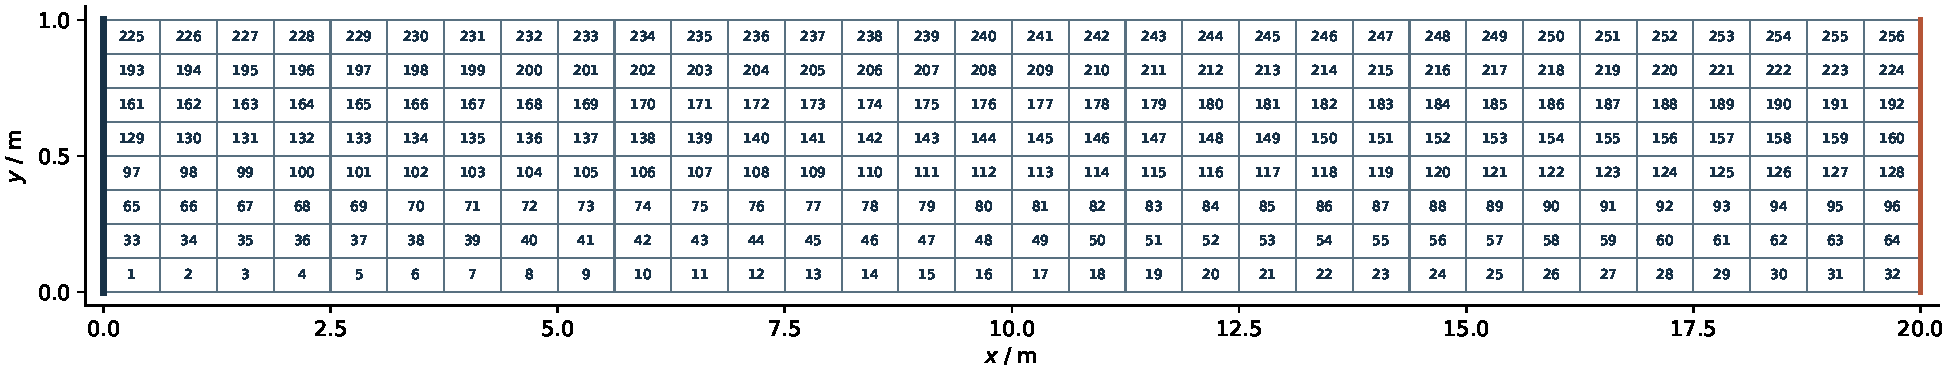
\includegraphics[width=\linewidth]{mesh_32x8.pdf}
\caption{$32\times8$网格，256个单元、297个节点。}
\end{figure}
\clearpage
\section{指定位置的位移}
节点位移求解后，任意单元内的位置不再引入新的未知量，而由形函数插值得到：
\begin{equation}
 u(x,y)=\sum_{a=1}^4N_a(x,y)u_a,\qquad
 v(x,y)=\sum_{a=1}^4N_a(x,y)v_a.
\end{equation}
对本题轴对齐矩形，先定位包含该点的单元，再计算
\[
\xi=2(x-x_L)/\Delta x-1,\qquad
\eta=2(y-y_B)/\Delta y-1.
\]
例如粗网格的$(10,1)$为第12单元右上角，$\xi=\eta=1$，四个形函数值为$(0,0,1,0)$。
第12单元连接节点$(13,14,23,22)$，因此该点位移直接等于节点23位移。
中性轴是整条$y=h/2=0.5\,\mathrm m$直线；中性轴挠度图在这条线上逐点插值。

\subsection{公共边的连续性}
Q4单元位移在公共边上连续，原因是相邻单元使用相同的两个端点位移。
例如公共竖边端点为A、B，以$t\in[0,1]$表示边上的位置，两侧都退化为
\[
u_{\rm edge}(t)=(1-t)u_A+tu_B,\qquad
v_{\rm edge}(t)=(1-t)v_A+tv_B.
\]
公共边上的位移一致；单元内部使用不同的其余节点，法向位移导数可以不同，沿边切向导数一致。

有限元弱形式包含位移的一阶导数积分，并不要求离散位移的一阶导数跨单元连续。
应变由导数构成，应力再由本构得到，因此原始单元应变和应力可以跳变。
\section{欧拉梁参考解}
令$w(x)$为中性轴竖向位移，向上为正；$z=y-h/2$为到中性轴的有符号距离。
采用小变形、平截面保持平面且垂直中性轴的欧拉梁假设。
截面转角$\theta\approx w'$，逆时针为正。截面中相对位置$(0,z)$转动后水平分量为
$-z\sin\theta\approx-z\theta$，因而在无轴向伸长的弯曲参考模型中
\begin{equation}
u=-zw',\qquad\varepsilon_{xx}=-zw'',\qquad\sigma_{xx}=-Ezw''.
\end{equation}
负号的几何含义是：正转角使上方点向左；本题$w'<0$，因此上方点向右。
相邻截面转角的变化引起伸长或缩短，单纯相同转角的刚体转动不会产生该轴向应变。

以向下端力大小$P>0$为参考加载。截开位置$x$，右端力臂为$L-x$。
定义截面应力矩$\mathcal M=\int_Az\sigma_{xx}\dd A$，由截面平衡及本构有
\begin{equation}
\mathcal M=P(L-x)=-EIw'',\qquad I=\int_Az^2\dd A=bh^3/12.
\end{equation}
用固定端$w(0)=w'(0)=0$积分两次：
\begin{align}
EIw'&=-P(Lx-x^2/2),\\
w(x)&=-\frac{Px^2(3L-x)}{6EI}.
\end{align}
原题为端部位移加载，取$\delta=0.1\,\mathrm m$，由$w(L)=-\delta$确定共同的解析端力：
\begin{equation}
P_{\rm EB}=\frac{3EI\delta}{L^3}=656.25\,\mathrm{kN}\quad(b=1\,\mathrm m),
\qquad
\boxed{w(x)=-\delta\frac{x^2(3L-x)}{2L^3}}.
\end{equation}
该端力是满足相同端挠度的解析参考，不是各套有限元网格各自的反力。
计算理论应力时也使用这个共同端力：
\begin{equation}
\sigma_{xx}^{\rm EB}(x,y)=\frac{P_{\rm EB}(L-x)}{I}(y-h/2),
\quad w(10)=-0.03125\,\mathrm m,
\quad \sigma_{xx}^{\rm EB}(10,1)=39.375\,\mathrm{MPa}.
\end{equation}

\section{挠度比较}
\begin{figure}[H]\centering
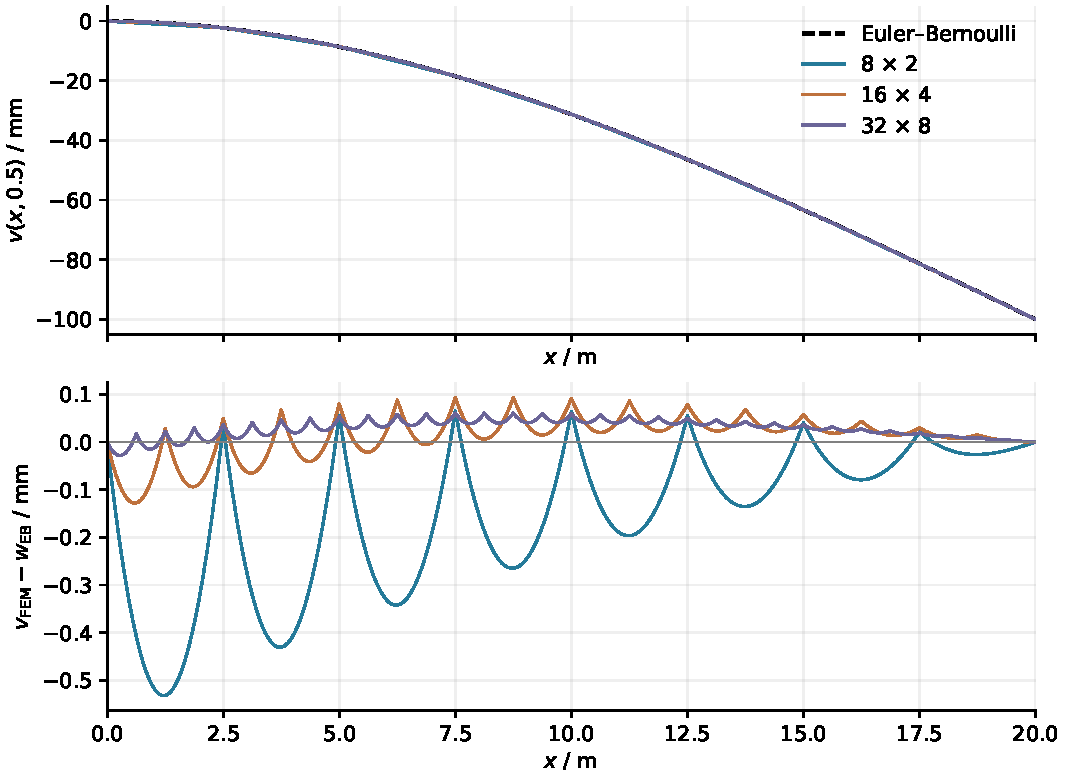
\includegraphics[width=.95\linewidth]{deflection.pdf}
\caption{中性轴挠度：三套Q4网格与欧拉梁解。上图为挠度，下图为有限元与欧拉梁的位移差；向下位移为负。}
\label{fig:deflection}
\end{figure}
中性轴位移采用单元形函数在641个横坐标处插值。
三套网格在$(10,0.5)$处的竖向位移依次为
\[
(-0.03118569,\;-0.03115850,\;-0.03119089)\,\mathrm m.
\]
与欧拉梁的差异均小于$0.1\,\mathrm{mm}$，但此点差异并非随网格单调变化。


\section{应变与应力计算}
指定位置的原始单元应变和应力由
\begin{equation}
\boldsymbol\varepsilon=B\mathbf d_e,\qquad
\boldsymbol\sigma=D\boldsymbol\varepsilon,\qquad
\sigma_{xx}=D_{11}\varepsilon_{xx}+D_{12}\varepsilon_{yy}
\end{equation}
得到。这里采用二维平面应变矩阵，不能用一维的$E\varepsilon_{xx}$替代。
粗网格第12单元在$(10,1)$的导数为
\[
(N_{a,x})=(0,0,0.4,-0.4)\,\mathrm{m^{-1}},\qquad
(N_{a,y})=(0,-2,2,0)\,\mathrm{m^{-1}}.
\]
因此$\varepsilon_{xx}=0.4(u_{23}-u_{22})=2.11776684\times10^{-4}$，
$\varepsilon_{yy}=2(v_{23}-v_{14})=-3.99839659\times10^{-5}$，
代入本构得到$\sigma_{xx}=55.0234\,\mathrm{MPa}$。

\subsection{整梁云图}
云图将每个位置的轴向应力映射为颜色：横纵坐标是梁内位置，色标单位为MPa；红色为正的拉应力，蓝色为负的压应力。
每个显示位置先定位单元，计算该点的$B$，取出该单元八个位移，再计算$DB\mathbf d_e$的第一分量。
靠近零应力的区域颜色较浅；颜色表示应力大小，不表示位移大小。

\begin{figure}[H]\centering
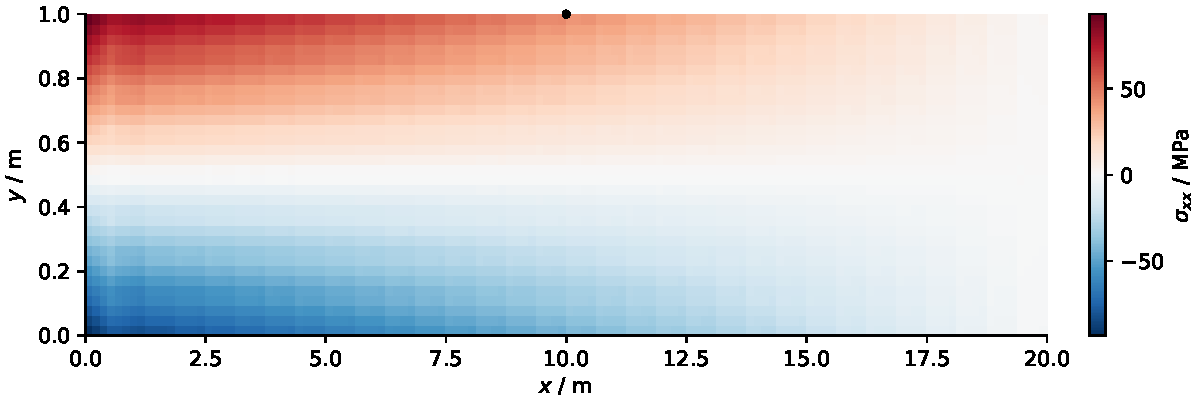
\includegraphics[width=\linewidth]{stress_contour.pdf}
\caption{最细$32\times8$网格的轴向应力。每个单元划分为$4\times4$个显示子区，
以子区中心的$DB\mathbf d_e$填色，不跨单元平均。纵向比例作显示放大，黑点为$(10,1)$。}
\label{fig:stress}
\end{figure}
拉应力为正、压应力为负。固定端附近存在边界约束效应，云图并不预设全域严格服从线性截面分布。
显示子区只用于提高云图的采样密度，并没有增加计算单元或位移自由度。

\subsection{指定点应力}
$(10,1)$同时属于左右两个单元。分别在两侧单元中直接代入该点的标准坐标，
保留两侧应力值，并以\textbf{等权算术平均}作为本次节点应力恢复约定。
\begin{table}[H]\centering
\caption{$(10,1)$处轴向应力；相对差异为$|\bar\sigma_{xx}-39.375|/39.375$。}
\begin{tabular}{rrrrr}\toprule 网格 & 左侧 / MPa & 右侧 / MPa & 平均 / MPa & 相对差异 / \%\\\midrule
$8\times2$ & 55.0234 & 41.6865 & 48.3550 & 22.81\\
$16\times4$ & 49.2550 & 42.5972 & 45.9261 & 16.64\\
$32\times8$ & 46.2799 & 42.9572 & 44.6186 & 13.32\\
\bottomrule\end{tabular}

\end{table}
\begin{figure}[H]\centering
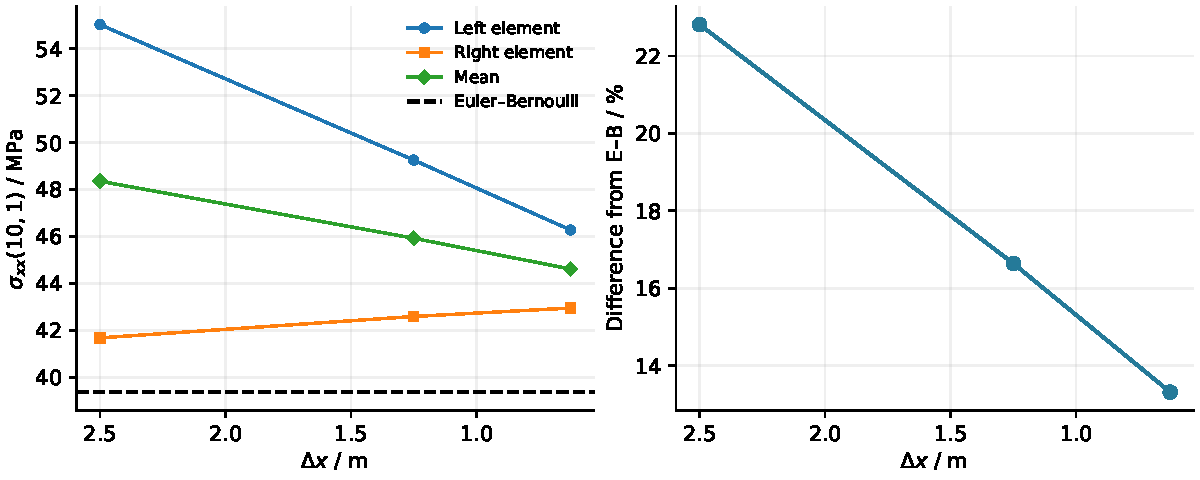
\includegraphics[width=\linewidth]{point_stress.pdf}
\caption{指定点的两侧及平均应力，与欧拉梁参考值的比较。横轴从左向右表示网格加密。}
\label{fig:point}
\end{figure}
两侧应力差从约$13.337$降至$6.658$、$3.323\,\mathrm{MPa}$。
平均应力逐渐靠近欧拉梁，但仅凭三套网格，不能确认二维连续体极限等于标准欧拉梁结果，
也不能把相对于梁理论的全部差异都归因于离散误差。

\section{误差分析}
\subsection{位移导数与弯曲离散}
位移的小差异在求导后可能成为较大的应变差异。边界位移插值连续，不代表单元斜率准确。
为说明多余剪切的来源，取一个宽度为$a$、中心横坐标为$x_c$的矩形单元。
常曲率弯曲的位移为$u=-\kappa xz$、$v=\kappa x^2/2$，其两个导数恰好抵消：
\[
u_{,y}=-\kappa x,\qquad v_{,x}=\kappa x,\qquad\gamma_{xy}=0.
\]
矩形Q4可以精确插值$xz$，但将二次函数$v$插值为单元内的一次函数，得到$v_{h,x}=\kappa x_c$。
因此离散剪应变为
\[
\gamma_{h,xy}=\kappa(x_c-x).
\]
它只在单元中心为零，其余位置产生本不该有的剪切能。
对本例积分得$U_{\rm extra}=bG\kappa^2 h_e a^3/24>0$，其中$h_e$为该单元高度。
附加能量使单元弯曲偏硬；网格加密减小$a$，可减轻这种影响。

\begin{table}[H]\centering
\caption{位移加载下的弯曲诊断。剪切能为$\frac12\int G\gamma_{xy}^2\dd V$，
挠度差为641个采样点相对于欧拉梁的最大绝对差。}
\begin{tabular}{rrrr}\toprule 网格 & 端力 / kN & 剪切能占比 / \% & 最大挠度差 / mm\\\midrule
$8\times2$ & 2347.295 & 67.28 & 0.5323\\
$16\times4$ & 1131.167 & 35.02 & 0.1281\\
$32\times8$ & 824.732 & 12.17 & 0.0611\\
\bottomrule\end{tabular}

\end{table}
反力随网格加密明显下降，剪切能占比也下降，支持粗网格偏硬的判断。
剪切能同时包含实际剪切与离散引入的额外剪切。

\subsection{模型约束与梁理论}
二维问题规定$\varepsilon_{zz}=0$，而标准欧拉梁使用一维轴向弹性关系。
远离端部，若局部近似$\sigma_{yy}=0$，由平面应变本构可得
\[
\varepsilon_{yy}=-\frac{\nu}{1-\nu}\varepsilon_{xx},\qquad
\sigma_{xx}=\frac{E}{1-\nu^2}\varepsilon_{xx}.
\]
因此，同一弯曲应变在该近似下对应更大的轴向应力。
把这一约束效应作为辅助量级估计，可得到
$39.375/(1-0.3^2)=43.2692\,\mathrm{MPa}$，比原梁参考高约$9.89\%$。


二维模型限制厚度方向变形，通常比一维梁更硬。两者又使用相同的端部位移，因此挠度曲线可以接近，但维持该位移所需的力和产生的应力仍有差别。固定端局部约束与网格误差也会影响结果。

\section{计算结论与复现}
三套网格均完成平面应变Q4位移求解和应力恢复。
最细网格在$(10,1)$的两侧平均轴向应力为$44.6186\,\mathrm{MPa}$，
相对标准欧拉梁高$13.32\%$；中性轴挠度曲线与梁理论接近。
网格加密减小了指定点的两侧应力跳跃，也降低了端部反力。
网格加密后应力跳跃减小；进一步加密可用于判断剩余差异中离散误差所占的比重。

\clearpage
\section{非线性扩展：J2弹塑性}
\subsection{插值与反力}
矩形Q4的四个形函数均由$(1\pm\xi)(1\pm\eta)/4$展开得到，包含$1,\xi,\eta,\xi\eta$。
由于矩形的$x$与$\xi$、截面高度$z=y-h/2$与$\eta$均为线性关系，
位移插值可写成$u_h=a_0+a_1x+a_2z+a_3xz$，$v_h$具有相同的基函数但系数不同。
这些系数由四个节点值确定，并非额外未知量。常曲率弯曲中$w''=\kappa$，
若取$w(0)=w'(0)=0$，积分得到$v=w=\kappa x^2/2$；截面转动则给出$u=-zw'=-\kappa xz$。
这里$z$仅表示截面内高度；下面的下标$zz$改指厚度方向。

反力由完整位移回代得到：$\mathbf r=K\mathbf d$（线弹性），
或由收敛应力积分得到$\mathbf r=\sum_e\int B^{\mathsf T}\boldsymbol\sigma\dd V$（无已知体力、面力时）。
右端合反力是所有右端竖向自由度之和。粗网格为节点9、18、27，
即$R_y=r_{18}+r_{36}+r_{54}$；中网格节点为17、34、51、68、85；
细网格节点为33、66、99、132、165、198、231、264、297。

\noindent\begin{minipage}{\linewidth}
\begin{lstlisting}
right_nodes = where(x == L)
vertical_dofs = 2 * right_nodes + 1
R_y = internal_force[vertical_dofs].sum()
\end{lstlisting}
\end{minipage}
上式伪代码使用从零开始的数组下标，报告节点编号从1开始。

\subsection{参数与三维材料状态}
沿用$E=210\,\mathrm{GPa}$、$\nu=0.30$；新增教学假设为
初始屈服应力$\sigma_{y0}=250\,\mathrm{MPa}$、硬化模量$H=1\,\mathrm{GPa}$。
这些参数未经材料试验标定。$H$定义为屈服应力对等效塑性应变的斜率，不是应力对总应变的斜率。
屈服面选用J2、流动法则选用关联流动、硬化选用线性各向同性硬化，均属于本构假设。

二维平面应变仍只求节点$u,v$，但材料点具有
$\varepsilon_{zz}=\varepsilon^e_{zz}+\varepsilon^p_{zz}=0$；两项可以分别非零。
因此必须保留$\sigma_{zz}$和$\varepsilon^p_{zz}$。
平面内的工程剪应变转换成三维张量时，$\varepsilon_{xy}=\gamma_{xy}/2$。
在本题对称假设下$xz,yz$剪切保持为零，程序用三维张量统一实现。

单轴拉伸试验中等效应力应等于轴向应力；J2进一步假定屈服不受静水压力影响，定义
\[
\mathbf s=\boldsymbol\sigma-\tfrac13\operatorname{tr}(\boldsymbol\sigma)I,
\quad q=\sqrt{\tfrac32\mathbf s:\mathbf s},
\quad \sigma_y(\alpha)=\sigma_{y0}+H\alpha,
\quad f=q-\sigma_y(\alpha).
\]
$f\le0$表示允许应力状态；弹性试算$f^{\rm tr}>0$时需产生塑性流动，使更新后的应力回到屈服面。
该条件不是由平衡方程推出，而是材料屈服及硬化假设。

\subsection{加载步与Newton试算}
$n$表示已收敛的加载步，$k$表示下一步内的Newton试算次数。两者不能混用。
例如右端位移从$-0.34$增至$-0.35\,\mathrm m$，这是一次加载；
在$-0.35\,\mathrm m$下反复修改内部自由节点位移，只是在寻找同一加载状态的平衡解。
右端规定值在这些试算中始终不变。

第$n$步结束后，保存位移$\mathbf d_n$及每个高斯点的材料状态
$\varepsilon^p_n,\alpha_n$。第$n+1$步的每次试算均执行
\[
\mathbf d^{(k)}_{n+1}\longrightarrow
\varepsilon^{(k)}_{n+1}=B\mathbf d^{(k)}_{e,n+1}
\longrightarrow
(\sigma^{(k)}_{n+1},\varepsilon^{p,(k)}_{n+1},\alpha^{(k)}_{n+1}).
\]
最后一个箭头始终以固定的$\varepsilon^p_n,\alpha_n$为起点。
其中候选塑性状态可以随$k$增大或减小，因为前几次候选尚未成为真实加载历史。
只有整体平衡收敛后，才将最后的候选保存为第$n+1$步的已确认状态。

例如$\alpha_n=0.001$，第一次试算得到$\Delta\alpha^{(0)}=0.0002$，
候选为$0.0012$；修正位移后重新计算得到$\Delta\alpha^{(1)}=0.00015$，
新候选应为$0.00115$，不能把上一次候选继续相加而得到$0.00135$。
后者把寻找平衡的数值试算当成了额外加载历史，会改变应力及反力。
若整个加载步失败，还须保留第$n$步状态，不能保存失败的候选。

\subsection{径向返回与分母中的$3G$}
剪切模量$G=E/[2(1+\nu)]=80.7692\,\mathrm{GPa}$，所以$3G=242.3077\,\mathrm{GPa}$。
这里是数字3乘以剪切模量，不是一个新材料参数。
先假设本步没有新增塑性，以总应变和上一加载步的塑性应变求弹性试算：
\[
\varepsilon^{e,\mathrm{tr}}=\varepsilon_{n+1}^{(k)}-\varepsilon^p_n,
\qquad \mathbf s^{\mathrm{tr}}=2G\operatorname{dev}(\varepsilon^{e,\mathrm{tr}}),
\qquad q^{\mathrm{tr}}=\sqrt{\tfrac32\mathbf s^{\mathrm{tr}}:\mathbf s^{\mathrm{tr}}}.
\]
若$q^{\mathrm{tr}}\le\sigma_{y0}+H\alpha_n$，保持塑性状态不变。
否则，关联J2流动法则及后向欧拉积分给出
\[
\Delta\varepsilon^p=\Delta\alpha\,\tfrac32
\frac{\mathbf s_{n+1}}{q_{n+1}}.
\]
各向同性弹性下，应力修正不改变偏应力方向，故
$\mathbf s_{n+1}/q_{n+1}=\mathbf s^{\mathrm{tr}}/q^{\mathrm{tr}}$。
塑性应变的迹为零，因此只修正偏应力：
\[
\mathbf s_{n+1}=\mathbf s^{\mathrm{tr}}-2G\Delta\varepsilon^p
=\left(1-\frac{3G\Delta\alpha}{q^{\mathrm{tr}}}\right)\mathbf s^{\mathrm{tr}}.
\]
其中$3G$来自$2G\times(3/2)$。代回等效应力定义，得到
\[
q_{n+1}=q^{\mathrm{tr}}-3G\Delta\alpha.
\]
同时屈服面随硬化扩大：$\sigma_{y,n+1}=\sigma_{y0}+H(\alpha_n+\Delta\alpha)$。
塑性修正后的应力必须满足$q_{n+1}=\sigma_{y,n+1}$，所以
\[
\boxed{\Delta\alpha=
\frac{q^{\mathrm{tr}}-\sigma_{y0}-H\alpha_n}{3G+H}.}
\]
分子是试算超过屈服面的应力量；分母将偏应力降低和屈服面扩大两种作用相加。
$\Delta\alpha$无量纲。这里的更新在每个高斯点独立完成。

\subsection{一致切线与整体位移修正}
将上述完整材料更新写成一个函数
\[
\boldsymbol\sigma_{n+1}=mathcal R(\boldsymbol\varepsilon_{n+1};
\boldsymbol\varepsilon^p_n,\alpha_n).
\]
分号后的状态固定。所谓一致切线，就是对这一个离散更新函数求导：
\[
C_t^{(k)}=\left.\frac{\partial\mathcal R}{\partial\boldsymbol\varepsilon}\right|_{
\varepsilon_{n+1}^{(k)};\,\varepsilon^p_n,\alpha_n},
\qquad \delta\boldsymbol\sigma\approx C_t^{(k)}\delta\boldsymbol\varepsilon.
\]
它回答：保持上一步历史不变，本次总应变稍微改变，应力会改变多少？
弹性区$C_t=D$；塑性区必须计入$\Delta\alpha$及返回方向随应变的变化，
不能一直沿用弹性矩阵$D$。程序求的是公式的解析导数，并非训练网络；
再用应变的中心差分检查该导数。

由内力和应变关系，逐层线性化得到
\[
\mathbf f_{\rm int}=\sum_e\int B^{\mathsf T}\boldsymbol\sigma\dd V,
\quad \delta\varepsilon=B\delta\mathbf d_e,
\quad K_t=\sum_e\int B^{\mathsf T}C_tB\dd V.
\]
本题自由位置没有已知外力，残差为$\mathbf r_f=\mathbf f_{{\rm int},f}$。
我们希望它变为零，于是Newton修正满足
\[
\mathbf r_f(\mathbf d^{(k)}+\delta\mathbf d)
\approx\mathbf r_f^{(k)}+K_{t,ff}^{(k)}\delta\mathbf d_f=0,
\qquad K_{t,ff}^{(k)}\delta\mathbf d_f=-\mathbf r_f^{(k)}.
\]
规定位置的修正为零；用稀疏直接解法解出自由位移修正，必要时通过线搜索缩小修正量。
随后重新计算应变、应力与残差。材料点的屈服条件满足，并不代表全梁已经平衡。

\noindent\begin{minipage}{\linewidth}
\begin{lstlisting}
for load_step in prescribed_displacements:
    impose_tip_displacement()
    for iteration in Newton:
        strain = B @ element_displacement
        stress, candidate, Ct = update(strain, old_state)
        internal_force, Kt = assemble(stress, Ct)
        if free_residual_is_small():
            old_state = candidate
            break
        correction = solve(Kt_ff, -internal_force_f)
        line_search(correction)
\end{lstlisting}
\end{minipage}
这里\code{old_state}在内层迭代期间固定，只有收敛分支才能替换。
线搜索的每次试算同样从该固定状态计算。

\subsection{工况与结果}
保留原题端位移$0.1\,\mathrm m$，另外扩展至$0.5\,\mathrm m$，共50步，每步$0.01\,\mathrm m$。
小应变、线性几何假设保持不变；该扩展不包含大转动或几何非线性。
三套网格在$0.1\,\mathrm m$均未屈服，反力与原线弹性结果一致。
\begin{table}[H]\centering
\caption{端位移$0.5\,\mathrm m$时的弹塑性结果。首次塑性按离散加载步记录。}
\begin{tabular}{rrrr}\toprule 网格 & 合反力大小 / kN & 最大$\alpha$ & 首次塑性位移 / m\\\midrule
$8\times2$ & 8407.268 & 0.001459 & 0.29\\
$16\times4$ & 5103.920 & 0.000841 & 0.35\\
$32\times8$ & 3801.481 & 0.000923 & 0.35\\
\bottomrule\end{tabular}
\end{table}
\begin{figure}[H]\centering
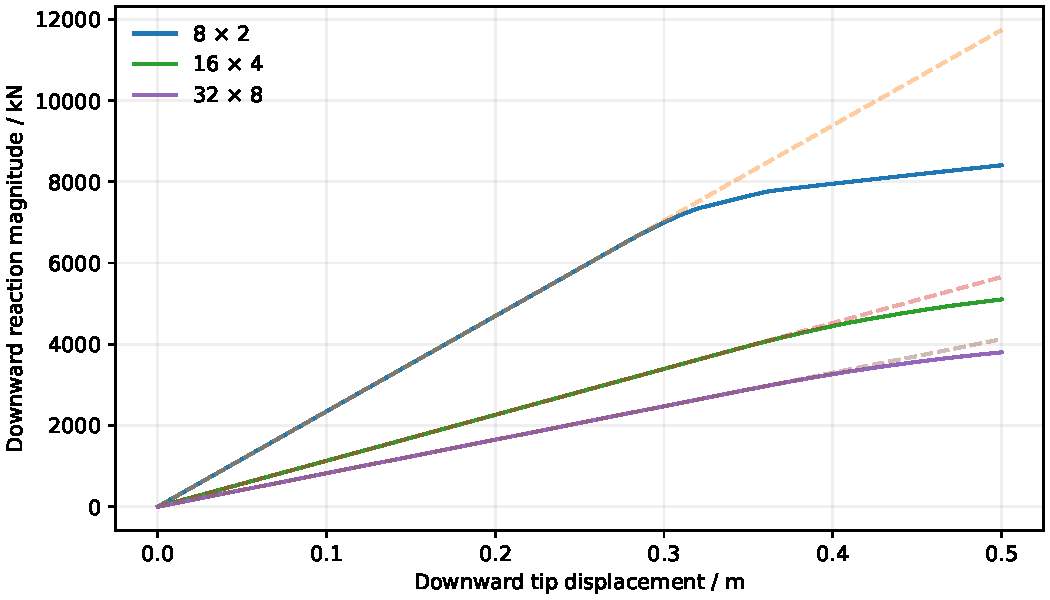
\includegraphics[width=.9\linewidth]{force_displacement.pdf}
\caption{三套网格的反力—位移曲线；虚线为各网格初始弹性刚度的延长线。}
\end{figure}
\begin{figure}[H]\centering
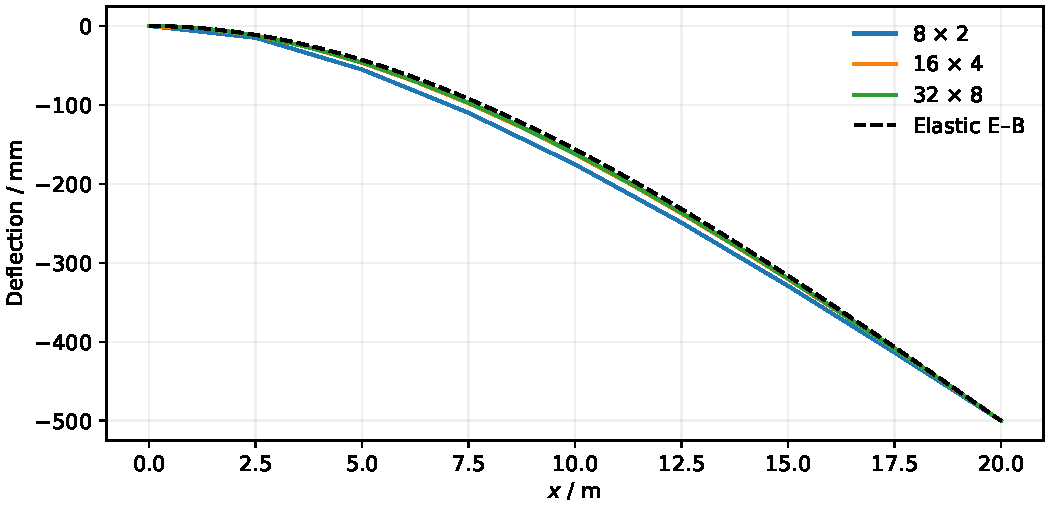
\includegraphics[width=.74\linewidth]{nonlinear_deflection.pdf}
\caption{端位移$0.5\,\mathrm m$的中性轴挠度；弹性欧拉梁只作为对照。}
\end{figure}
\begin{figure}[H]\centering
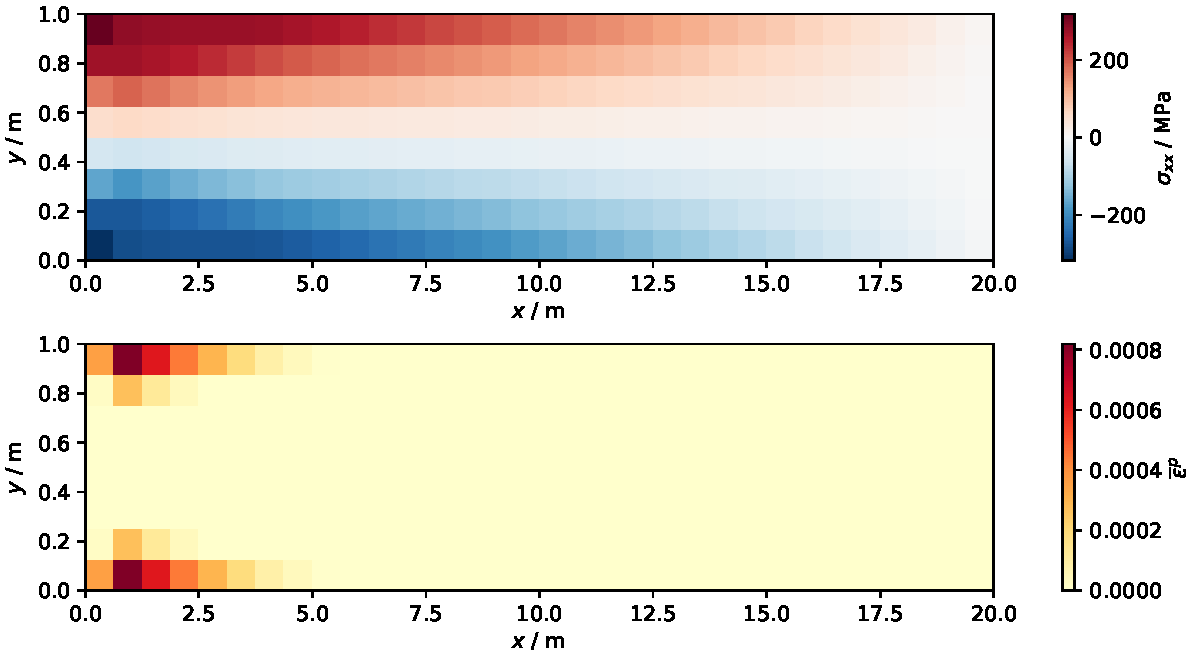
\includegraphics[width=.74\linewidth]{plastic_cloud.pdf}
\caption{最细网格在端位移$0.5\,\mathrm m$时的轴向应力及等效塑性应变。
每个单元以四个高斯点的均值填色，纵向比例作显示放大。}
\end{figure}
\begin{table}[H]\centering
\caption{$0.5\,\mathrm m$时$(10,1)$的轴向应力；弹性欧拉梁对照为$196.875\,\mathrm{MPa}$。}
\begin{tabular}{rrrr}\toprule 网格 & 左侧 / MPa & 右侧 / MPa & 平均 / MPa\\\midrule
$8\times2$ & 196.638 & 149.113 & 172.876\\
$16\times4$ & 222.243 & 192.199 & 207.221\\
$32\times8$ & 213.321 & 198.005 & 205.663\\
\bottomrule\end{tabular}
\end{table}
塑性状态保存在高斯点。指定边界点应力由同一单元四个高斯点应力双线性外推，再将左右单元值平均。
这与线弹性章节直接在顶点求导的方式不同，不能把两者的恢复差异当作材料非线性效应。
此工况中指定点可能仍处于弹性区，反力曲线和塑性应变云图用于判断全梁是否出现塑性。
线弹性梁不包含塑性，因此与其差异同时包含模型差异及网格误差。

材料一致切线已用中心差分验证，弹性极限反力与原求解器核对；
三套网格每一步均检查自由方程残差和总力平衡。最细网格最多5次Newton修正，
全试验最大相对残差小于$10^{-8}$。最细网格改为100步后，终点反力为$3801.586\,\mathrm{kN}$，较50步变化约$0.0028\%$。不同网格首次发现塑性的位移不同，尚需更细网格及加载步长验证屈服起点。

\clearpage\appendix
\section{ID与IEN表}
表中左右两组分别列出独立的节点或单元记录。
ID下标$u,v$表示位移方向，$g_u,g_v$表示未缩减的全局自由度编号。
已知位移按节点所在边界赋值：左端$u=v=0$，右端$v=-0.1\,\mathrm m$。
IEN在正文定义为$4\times n_e$；下面每条记录对应其中一列，即一个单元。
\setlength{\tabcolsep}{4pt}
\subsection{$8\times2$ 网格}
\subsubsection*{ID：节点与自由方程编号}
\small\begin{longtable}{rrrrr@{\qquad}rrrrr}
\toprule 节点 & $g_u$ & $g_v$ & ID$_u$ & ID$_v$ & 节点 & $g_u$ & $g_v$ & ID$_u$ & ID$_v$ \\ \midrule\endhead
1 & 1 & 2 & 0 & 0 & 15 & 29 & 30 & 24 & 25 \\
2 & 3 & 4 & 1 & 2 & 16 & 31 & 32 & 26 & 27 \\
3 & 5 & 6 & 3 & 4 & 17 & 33 & 34 & 28 & 29 \\
4 & 7 & 8 & 5 & 6 & 18 & 35 & 36 & 30 & 0 \\
5 & 9 & 10 & 7 & 8 & 19 & 37 & 38 & 0 & 0 \\
6 & 11 & 12 & 9 & 10 & 20 & 39 & 40 & 31 & 32 \\
7 & 13 & 14 & 11 & 12 & 21 & 41 & 42 & 33 & 34 \\
8 & 15 & 16 & 13 & 14 & 22 & 43 & 44 & 35 & 36 \\
9 & 17 & 18 & 15 & 0 & 23 & 45 & 46 & 37 & 38 \\
10 & 19 & 20 & 0 & 0 & 24 & 47 & 48 & 39 & 40 \\
11 & 21 & 22 & 16 & 17 & 25 & 49 & 50 & 41 & 42 \\
12 & 23 & 24 & 18 & 19 & 26 & 51 & 52 & 43 & 44 \\
13 & 25 & 26 & 20 & 21 & 27 & 53 & 54 & 45 & 0 \\
14 & 27 & 28 & 22 & 23 &  &  &  &  &  \\
\bottomrule\end{longtable}\normalsize
\subsubsection*{IEN：单元与全局节点编号}
\small\begin{longtable}{rrrrr@{\qquad}rrrrr}
\toprule 单元 & $n_1$ & $n_2$ & $n_3$ & $n_4$ & 单元 & $n_1$ & $n_2$ & $n_3$ & $n_4$ \\ \midrule\endhead
1 & 1 & 2 & 11 & 10 & 9 & 10 & 11 & 20 & 19 \\
2 & 2 & 3 & 12 & 11 & 10 & 11 & 12 & 21 & 20 \\
3 & 3 & 4 & 13 & 12 & 11 & 12 & 13 & 22 & 21 \\
4 & 4 & 5 & 14 & 13 & 12 & 13 & 14 & 23 & 22 \\
5 & 5 & 6 & 15 & 14 & 13 & 14 & 15 & 24 & 23 \\
6 & 6 & 7 & 16 & 15 & 14 & 15 & 16 & 25 & 24 \\
7 & 7 & 8 & 17 & 16 & 15 & 16 & 17 & 26 & 25 \\
8 & 8 & 9 & 18 & 17 & 16 & 17 & 18 & 27 & 26 \\
\bottomrule\end{longtable}\normalsize
\clearpage
\subsection{$16\times4$ 网格}
\subsubsection*{ID：节点与自由方程编号}
\small\begin{longtable}{rrrrr@{\qquad}rrrrr}
\toprule 节点 & $g_u$ & $g_v$ & ID$_u$ & ID$_v$ & 节点 & $g_u$ & $g_v$ & ID$_u$ & ID$_v$ \\ \midrule\endhead
1 & 1 & 2 & 0 & 0 & 44 & 87 & 88 & 79 & 80 \\
2 & 3 & 4 & 1 & 2 & 45 & 89 & 90 & 81 & 82 \\
3 & 5 & 6 & 3 & 4 & 46 & 91 & 92 & 83 & 84 \\
4 & 7 & 8 & 5 & 6 & 47 & 93 & 94 & 85 & 86 \\
5 & 9 & 10 & 7 & 8 & 48 & 95 & 96 & 87 & 88 \\
6 & 11 & 12 & 9 & 10 & 49 & 97 & 98 & 89 & 90 \\
7 & 13 & 14 & 11 & 12 & 50 & 99 & 100 & 91 & 92 \\
8 & 15 & 16 & 13 & 14 & 51 & 101 & 102 & 93 & 0 \\
9 & 17 & 18 & 15 & 16 & 52 & 103 & 104 & 0 & 0 \\
10 & 19 & 20 & 17 & 18 & 53 & 105 & 106 & 94 & 95 \\
11 & 21 & 22 & 19 & 20 & 54 & 107 & 108 & 96 & 97 \\
12 & 23 & 24 & 21 & 22 & 55 & 109 & 110 & 98 & 99 \\
13 & 25 & 26 & 23 & 24 & 56 & 111 & 112 & 100 & 101 \\
14 & 27 & 28 & 25 & 26 & 57 & 113 & 114 & 102 & 103 \\
15 & 29 & 30 & 27 & 28 & 58 & 115 & 116 & 104 & 105 \\
16 & 31 & 32 & 29 & 30 & 59 & 117 & 118 & 106 & 107 \\
17 & 33 & 34 & 31 & 0 & 60 & 119 & 120 & 108 & 109 \\
18 & 35 & 36 & 0 & 0 & 61 & 121 & 122 & 110 & 111 \\
19 & 37 & 38 & 32 & 33 & 62 & 123 & 124 & 112 & 113 \\
20 & 39 & 40 & 34 & 35 & 63 & 125 & 126 & 114 & 115 \\
21 & 41 & 42 & 36 & 37 & 64 & 127 & 128 & 116 & 117 \\
22 & 43 & 44 & 38 & 39 & 65 & 129 & 130 & 118 & 119 \\
23 & 45 & 46 & 40 & 41 & 66 & 131 & 132 & 120 & 121 \\
24 & 47 & 48 & 42 & 43 & 67 & 133 & 134 & 122 & 123 \\
25 & 49 & 50 & 44 & 45 & 68 & 135 & 136 & 124 & 0 \\
26 & 51 & 52 & 46 & 47 & 69 & 137 & 138 & 0 & 0 \\
27 & 53 & 54 & 48 & 49 & 70 & 139 & 140 & 125 & 126 \\
28 & 55 & 56 & 50 & 51 & 71 & 141 & 142 & 127 & 128 \\
29 & 57 & 58 & 52 & 53 & 72 & 143 & 144 & 129 & 130 \\
30 & 59 & 60 & 54 & 55 & 73 & 145 & 146 & 131 & 132 \\
31 & 61 & 62 & 56 & 57 & 74 & 147 & 148 & 133 & 134 \\
32 & 63 & 64 & 58 & 59 & 75 & 149 & 150 & 135 & 136 \\
33 & 65 & 66 & 60 & 61 & 76 & 151 & 152 & 137 & 138 \\
34 & 67 & 68 & 62 & 0 & 77 & 153 & 154 & 139 & 140 \\
35 & 69 & 70 & 0 & 0 & 78 & 155 & 156 & 141 & 142 \\
36 & 71 & 72 & 63 & 64 & 79 & 157 & 158 & 143 & 144 \\
37 & 73 & 74 & 65 & 66 & 80 & 159 & 160 & 145 & 146 \\
38 & 75 & 76 & 67 & 68 & 81 & 161 & 162 & 147 & 148 \\
39 & 77 & 78 & 69 & 70 & 82 & 163 & 164 & 149 & 150 \\
40 & 79 & 80 & 71 & 72 & 83 & 165 & 166 & 151 & 152 \\
41 & 81 & 82 & 73 & 74 & 84 & 167 & 168 & 153 & 154 \\
42 & 83 & 84 & 75 & 76 & 85 & 169 & 170 & 155 & 0 \\
43 & 85 & 86 & 77 & 78 &  &  &  &  &  \\
\bottomrule\end{longtable}\normalsize
\subsubsection*{IEN：单元与全局节点编号}
\small\begin{longtable}{rrrrr@{\qquad}rrrrr}
\toprule 单元 & $n_1$ & $n_2$ & $n_3$ & $n_4$ & 单元 & $n_1$ & $n_2$ & $n_3$ & $n_4$ \\ \midrule\endhead
1 & 1 & 2 & 19 & 18 & 33 & 35 & 36 & 53 & 52 \\
2 & 2 & 3 & 20 & 19 & 34 & 36 & 37 & 54 & 53 \\
3 & 3 & 4 & 21 & 20 & 35 & 37 & 38 & 55 & 54 \\
4 & 4 & 5 & 22 & 21 & 36 & 38 & 39 & 56 & 55 \\
5 & 5 & 6 & 23 & 22 & 37 & 39 & 40 & 57 & 56 \\
6 & 6 & 7 & 24 & 23 & 38 & 40 & 41 & 58 & 57 \\
7 & 7 & 8 & 25 & 24 & 39 & 41 & 42 & 59 & 58 \\
8 & 8 & 9 & 26 & 25 & 40 & 42 & 43 & 60 & 59 \\
9 & 9 & 10 & 27 & 26 & 41 & 43 & 44 & 61 & 60 \\
10 & 10 & 11 & 28 & 27 & 42 & 44 & 45 & 62 & 61 \\
11 & 11 & 12 & 29 & 28 & 43 & 45 & 46 & 63 & 62 \\
12 & 12 & 13 & 30 & 29 & 44 & 46 & 47 & 64 & 63 \\
13 & 13 & 14 & 31 & 30 & 45 & 47 & 48 & 65 & 64 \\
14 & 14 & 15 & 32 & 31 & 46 & 48 & 49 & 66 & 65 \\
15 & 15 & 16 & 33 & 32 & 47 & 49 & 50 & 67 & 66 \\
16 & 16 & 17 & 34 & 33 & 48 & 50 & 51 & 68 & 67 \\
17 & 18 & 19 & 36 & 35 & 49 & 52 & 53 & 70 & 69 \\
18 & 19 & 20 & 37 & 36 & 50 & 53 & 54 & 71 & 70 \\
19 & 20 & 21 & 38 & 37 & 51 & 54 & 55 & 72 & 71 \\
20 & 21 & 22 & 39 & 38 & 52 & 55 & 56 & 73 & 72 \\
21 & 22 & 23 & 40 & 39 & 53 & 56 & 57 & 74 & 73 \\
22 & 23 & 24 & 41 & 40 & 54 & 57 & 58 & 75 & 74 \\
23 & 24 & 25 & 42 & 41 & 55 & 58 & 59 & 76 & 75 \\
24 & 25 & 26 & 43 & 42 & 56 & 59 & 60 & 77 & 76 \\
25 & 26 & 27 & 44 & 43 & 57 & 60 & 61 & 78 & 77 \\
26 & 27 & 28 & 45 & 44 & 58 & 61 & 62 & 79 & 78 \\
27 & 28 & 29 & 46 & 45 & 59 & 62 & 63 & 80 & 79 \\
28 & 29 & 30 & 47 & 46 & 60 & 63 & 64 & 81 & 80 \\
29 & 30 & 31 & 48 & 47 & 61 & 64 & 65 & 82 & 81 \\
30 & 31 & 32 & 49 & 48 & 62 & 65 & 66 & 83 & 82 \\
31 & 32 & 33 & 50 & 49 & 63 & 66 & 67 & 84 & 83 \\
32 & 33 & 34 & 51 & 50 & 64 & 67 & 68 & 85 & 84 \\
\bottomrule\end{longtable}\normalsize
\clearpage
\subsection{$32\times8$ 网格}
\subsubsection*{ID：节点与自由方程编号}
\small\begin{longtable}{rrrrr@{\qquad}rrrrr}
\toprule 节点 & $g_u$ & $g_v$ & ID$_u$ & ID$_v$ & 节点 & $g_u$ & $g_v$ & ID$_u$ & ID$_v$ \\ \midrule\endhead
1 & 1 & 2 & 0 & 0 & 150 & 299 & 300 & 285 & 286 \\
2 & 3 & 4 & 1 & 2 & 151 & 301 & 302 & 287 & 288 \\
3 & 5 & 6 & 3 & 4 & 152 & 303 & 304 & 289 & 290 \\
4 & 7 & 8 & 5 & 6 & 153 & 305 & 306 & 291 & 292 \\
5 & 9 & 10 & 7 & 8 & 154 & 307 & 308 & 293 & 294 \\
6 & 11 & 12 & 9 & 10 & 155 & 309 & 310 & 295 & 296 \\
7 & 13 & 14 & 11 & 12 & 156 & 311 & 312 & 297 & 298 \\
8 & 15 & 16 & 13 & 14 & 157 & 313 & 314 & 299 & 300 \\
9 & 17 & 18 & 15 & 16 & 158 & 315 & 316 & 301 & 302 \\
10 & 19 & 20 & 17 & 18 & 159 & 317 & 318 & 303 & 304 \\
11 & 21 & 22 & 19 & 20 & 160 & 319 & 320 & 305 & 306 \\
12 & 23 & 24 & 21 & 22 & 161 & 321 & 322 & 307 & 308 \\
13 & 25 & 26 & 23 & 24 & 162 & 323 & 324 & 309 & 310 \\
14 & 27 & 28 & 25 & 26 & 163 & 325 & 326 & 311 & 312 \\
15 & 29 & 30 & 27 & 28 & 164 & 327 & 328 & 313 & 314 \\
16 & 31 & 32 & 29 & 30 & 165 & 329 & 330 & 315 & 0 \\
17 & 33 & 34 & 31 & 32 & 166 & 331 & 332 & 0 & 0 \\
18 & 35 & 36 & 33 & 34 & 167 & 333 & 334 & 316 & 317 \\
19 & 37 & 38 & 35 & 36 & 168 & 335 & 336 & 318 & 319 \\
20 & 39 & 40 & 37 & 38 & 169 & 337 & 338 & 320 & 321 \\
21 & 41 & 42 & 39 & 40 & 170 & 339 & 340 & 322 & 323 \\
22 & 43 & 44 & 41 & 42 & 171 & 341 & 342 & 324 & 325 \\
23 & 45 & 46 & 43 & 44 & 172 & 343 & 344 & 326 & 327 \\
24 & 47 & 48 & 45 & 46 & 173 & 345 & 346 & 328 & 329 \\
25 & 49 & 50 & 47 & 48 & 174 & 347 & 348 & 330 & 331 \\
26 & 51 & 52 & 49 & 50 & 175 & 349 & 350 & 332 & 333 \\
27 & 53 & 54 & 51 & 52 & 176 & 351 & 352 & 334 & 335 \\
28 & 55 & 56 & 53 & 54 & 177 & 353 & 354 & 336 & 337 \\
29 & 57 & 58 & 55 & 56 & 178 & 355 & 356 & 338 & 339 \\
30 & 59 & 60 & 57 & 58 & 179 & 357 & 358 & 340 & 341 \\
31 & 61 & 62 & 59 & 60 & 180 & 359 & 360 & 342 & 343 \\
32 & 63 & 64 & 61 & 62 & 181 & 361 & 362 & 344 & 345 \\
33 & 65 & 66 & 63 & 0 & 182 & 363 & 364 & 346 & 347 \\
34 & 67 & 68 & 0 & 0 & 183 & 365 & 366 & 348 & 349 \\
35 & 69 & 70 & 64 & 65 & 184 & 367 & 368 & 350 & 351 \\
36 & 71 & 72 & 66 & 67 & 185 & 369 & 370 & 352 & 353 \\
37 & 73 & 74 & 68 & 69 & 186 & 371 & 372 & 354 & 355 \\
38 & 75 & 76 & 70 & 71 & 187 & 373 & 374 & 356 & 357 \\
39 & 77 & 78 & 72 & 73 & 188 & 375 & 376 & 358 & 359 \\
40 & 79 & 80 & 74 & 75 & 189 & 377 & 378 & 360 & 361 \\
41 & 81 & 82 & 76 & 77 & 190 & 379 & 380 & 362 & 363 \\
42 & 83 & 84 & 78 & 79 & 191 & 381 & 382 & 364 & 365 \\
43 & 85 & 86 & 80 & 81 & 192 & 383 & 384 & 366 & 367 \\
44 & 87 & 88 & 82 & 83 & 193 & 385 & 386 & 368 & 369 \\
45 & 89 & 90 & 84 & 85 & 194 & 387 & 388 & 370 & 371 \\
46 & 91 & 92 & 86 & 87 & 195 & 389 & 390 & 372 & 373 \\
47 & 93 & 94 & 88 & 89 & 196 & 391 & 392 & 374 & 375 \\
48 & 95 & 96 & 90 & 91 & 197 & 393 & 394 & 376 & 377 \\
49 & 97 & 98 & 92 & 93 & 198 & 395 & 396 & 378 & 0 \\
50 & 99 & 100 & 94 & 95 & 199 & 397 & 398 & 0 & 0 \\
51 & 101 & 102 & 96 & 97 & 200 & 399 & 400 & 379 & 380 \\
52 & 103 & 104 & 98 & 99 & 201 & 401 & 402 & 381 & 382 \\
53 & 105 & 106 & 100 & 101 & 202 & 403 & 404 & 383 & 384 \\
54 & 107 & 108 & 102 & 103 & 203 & 405 & 406 & 385 & 386 \\
55 & 109 & 110 & 104 & 105 & 204 & 407 & 408 & 387 & 388 \\
56 & 111 & 112 & 106 & 107 & 205 & 409 & 410 & 389 & 390 \\
57 & 113 & 114 & 108 & 109 & 206 & 411 & 412 & 391 & 392 \\
58 & 115 & 116 & 110 & 111 & 207 & 413 & 414 & 393 & 394 \\
59 & 117 & 118 & 112 & 113 & 208 & 415 & 416 & 395 & 396 \\
60 & 119 & 120 & 114 & 115 & 209 & 417 & 418 & 397 & 398 \\
61 & 121 & 122 & 116 & 117 & 210 & 419 & 420 & 399 & 400 \\
62 & 123 & 124 & 118 & 119 & 211 & 421 & 422 & 401 & 402 \\
63 & 125 & 126 & 120 & 121 & 212 & 423 & 424 & 403 & 404 \\
64 & 127 & 128 & 122 & 123 & 213 & 425 & 426 & 405 & 406 \\
65 & 129 & 130 & 124 & 125 & 214 & 427 & 428 & 407 & 408 \\
66 & 131 & 132 & 126 & 0 & 215 & 429 & 430 & 409 & 410 \\
67 & 133 & 134 & 0 & 0 & 216 & 431 & 432 & 411 & 412 \\
68 & 135 & 136 & 127 & 128 & 217 & 433 & 434 & 413 & 414 \\
69 & 137 & 138 & 129 & 130 & 218 & 435 & 436 & 415 & 416 \\
70 & 139 & 140 & 131 & 132 & 219 & 437 & 438 & 417 & 418 \\
71 & 141 & 142 & 133 & 134 & 220 & 439 & 440 & 419 & 420 \\
72 & 143 & 144 & 135 & 136 & 221 & 441 & 442 & 421 & 422 \\
73 & 145 & 146 & 137 & 138 & 222 & 443 & 444 & 423 & 424 \\
74 & 147 & 148 & 139 & 140 & 223 & 445 & 446 & 425 & 426 \\
75 & 149 & 150 & 141 & 142 & 224 & 447 & 448 & 427 & 428 \\
76 & 151 & 152 & 143 & 144 & 225 & 449 & 450 & 429 & 430 \\
77 & 153 & 154 & 145 & 146 & 226 & 451 & 452 & 431 & 432 \\
78 & 155 & 156 & 147 & 148 & 227 & 453 & 454 & 433 & 434 \\
79 & 157 & 158 & 149 & 150 & 228 & 455 & 456 & 435 & 436 \\
80 & 159 & 160 & 151 & 152 & 229 & 457 & 458 & 437 & 438 \\
81 & 161 & 162 & 153 & 154 & 230 & 459 & 460 & 439 & 440 \\
82 & 163 & 164 & 155 & 156 & 231 & 461 & 462 & 441 & 0 \\
83 & 165 & 166 & 157 & 158 & 232 & 463 & 464 & 0 & 0 \\
84 & 167 & 168 & 159 & 160 & 233 & 465 & 466 & 442 & 443 \\
85 & 169 & 170 & 161 & 162 & 234 & 467 & 468 & 444 & 445 \\
86 & 171 & 172 & 163 & 164 & 235 & 469 & 470 & 446 & 447 \\
87 & 173 & 174 & 165 & 166 & 236 & 471 & 472 & 448 & 449 \\
88 & 175 & 176 & 167 & 168 & 237 & 473 & 474 & 450 & 451 \\
89 & 177 & 178 & 169 & 170 & 238 & 475 & 476 & 452 & 453 \\
90 & 179 & 180 & 171 & 172 & 239 & 477 & 478 & 454 & 455 \\
91 & 181 & 182 & 173 & 174 & 240 & 479 & 480 & 456 & 457 \\
92 & 183 & 184 & 175 & 176 & 241 & 481 & 482 & 458 & 459 \\
93 & 185 & 186 & 177 & 178 & 242 & 483 & 484 & 460 & 461 \\
94 & 187 & 188 & 179 & 180 & 243 & 485 & 486 & 462 & 463 \\
95 & 189 & 190 & 181 & 182 & 244 & 487 & 488 & 464 & 465 \\
96 & 191 & 192 & 183 & 184 & 245 & 489 & 490 & 466 & 467 \\
97 & 193 & 194 & 185 & 186 & 246 & 491 & 492 & 468 & 469 \\
98 & 195 & 196 & 187 & 188 & 247 & 493 & 494 & 470 & 471 \\
99 & 197 & 198 & 189 & 0 & 248 & 495 & 496 & 472 & 473 \\
100 & 199 & 200 & 0 & 0 & 249 & 497 & 498 & 474 & 475 \\
101 & 201 & 202 & 190 & 191 & 250 & 499 & 500 & 476 & 477 \\
102 & 203 & 204 & 192 & 193 & 251 & 501 & 502 & 478 & 479 \\
103 & 205 & 206 & 194 & 195 & 252 & 503 & 504 & 480 & 481 \\
104 & 207 & 208 & 196 & 197 & 253 & 505 & 506 & 482 & 483 \\
105 & 209 & 210 & 198 & 199 & 254 & 507 & 508 & 484 & 485 \\
106 & 211 & 212 & 200 & 201 & 255 & 509 & 510 & 486 & 487 \\
107 & 213 & 214 & 202 & 203 & 256 & 511 & 512 & 488 & 489 \\
108 & 215 & 216 & 204 & 205 & 257 & 513 & 514 & 490 & 491 \\
109 & 217 & 218 & 206 & 207 & 258 & 515 & 516 & 492 & 493 \\
110 & 219 & 220 & 208 & 209 & 259 & 517 & 518 & 494 & 495 \\
111 & 221 & 222 & 210 & 211 & 260 & 519 & 520 & 496 & 497 \\
112 & 223 & 224 & 212 & 213 & 261 & 521 & 522 & 498 & 499 \\
113 & 225 & 226 & 214 & 215 & 262 & 523 & 524 & 500 & 501 \\
114 & 227 & 228 & 216 & 217 & 263 & 525 & 526 & 502 & 503 \\
115 & 229 & 230 & 218 & 219 & 264 & 527 & 528 & 504 & 0 \\
116 & 231 & 232 & 220 & 221 & 265 & 529 & 530 & 0 & 0 \\
117 & 233 & 234 & 222 & 223 & 266 & 531 & 532 & 505 & 506 \\
118 & 235 & 236 & 224 & 225 & 267 & 533 & 534 & 507 & 508 \\
119 & 237 & 238 & 226 & 227 & 268 & 535 & 536 & 509 & 510 \\
120 & 239 & 240 & 228 & 229 & 269 & 537 & 538 & 511 & 512 \\
121 & 241 & 242 & 230 & 231 & 270 & 539 & 540 & 513 & 514 \\
122 & 243 & 244 & 232 & 233 & 271 & 541 & 542 & 515 & 516 \\
123 & 245 & 246 & 234 & 235 & 272 & 543 & 544 & 517 & 518 \\
124 & 247 & 248 & 236 & 237 & 273 & 545 & 546 & 519 & 520 \\
125 & 249 & 250 & 238 & 239 & 274 & 547 & 548 & 521 & 522 \\
126 & 251 & 252 & 240 & 241 & 275 & 549 & 550 & 523 & 524 \\
127 & 253 & 254 & 242 & 243 & 276 & 551 & 552 & 525 & 526 \\
128 & 255 & 256 & 244 & 245 & 277 & 553 & 554 & 527 & 528 \\
129 & 257 & 258 & 246 & 247 & 278 & 555 & 556 & 529 & 530 \\
130 & 259 & 260 & 248 & 249 & 279 & 557 & 558 & 531 & 532 \\
131 & 261 & 262 & 250 & 251 & 280 & 559 & 560 & 533 & 534 \\
132 & 263 & 264 & 252 & 0 & 281 & 561 & 562 & 535 & 536 \\
133 & 265 & 266 & 0 & 0 & 282 & 563 & 564 & 537 & 538 \\
134 & 267 & 268 & 253 & 254 & 283 & 565 & 566 & 539 & 540 \\
135 & 269 & 270 & 255 & 256 & 284 & 567 & 568 & 541 & 542 \\
136 & 271 & 272 & 257 & 258 & 285 & 569 & 570 & 543 & 544 \\
137 & 273 & 274 & 259 & 260 & 286 & 571 & 572 & 545 & 546 \\
138 & 275 & 276 & 261 & 262 & 287 & 573 & 574 & 547 & 548 \\
139 & 277 & 278 & 263 & 264 & 288 & 575 & 576 & 549 & 550 \\
140 & 279 & 280 & 265 & 266 & 289 & 577 & 578 & 551 & 552 \\
141 & 281 & 282 & 267 & 268 & 290 & 579 & 580 & 553 & 554 \\
142 & 283 & 284 & 269 & 270 & 291 & 581 & 582 & 555 & 556 \\
143 & 285 & 286 & 271 & 272 & 292 & 583 & 584 & 557 & 558 \\
144 & 287 & 288 & 273 & 274 & 293 & 585 & 586 & 559 & 560 \\
145 & 289 & 290 & 275 & 276 & 294 & 587 & 588 & 561 & 562 \\
146 & 291 & 292 & 277 & 278 & 295 & 589 & 590 & 563 & 564 \\
147 & 293 & 294 & 279 & 280 & 296 & 591 & 592 & 565 & 566 \\
148 & 295 & 296 & 281 & 282 & 297 & 593 & 594 & 567 & 0 \\
149 & 297 & 298 & 283 & 284 &  &  &  &  &  \\
\bottomrule\end{longtable}\normalsize
\subsubsection*{IEN：单元与全局节点编号}
\small\begin{longtable}{rrrrr@{\qquad}rrrrr}
\toprule 单元 & $n_1$ & $n_2$ & $n_3$ & $n_4$ & 单元 & $n_1$ & $n_2$ & $n_3$ & $n_4$ \\ \midrule\endhead
1 & 1 & 2 & 35 & 34 & 129 & 133 & 134 & 167 & 166 \\
2 & 2 & 3 & 36 & 35 & 130 & 134 & 135 & 168 & 167 \\
3 & 3 & 4 & 37 & 36 & 131 & 135 & 136 & 169 & 168 \\
4 & 4 & 5 & 38 & 37 & 132 & 136 & 137 & 170 & 169 \\
5 & 5 & 6 & 39 & 38 & 133 & 137 & 138 & 171 & 170 \\
6 & 6 & 7 & 40 & 39 & 134 & 138 & 139 & 172 & 171 \\
7 & 7 & 8 & 41 & 40 & 135 & 139 & 140 & 173 & 172 \\
8 & 8 & 9 & 42 & 41 & 136 & 140 & 141 & 174 & 173 \\
9 & 9 & 10 & 43 & 42 & 137 & 141 & 142 & 175 & 174 \\
10 & 10 & 11 & 44 & 43 & 138 & 142 & 143 & 176 & 175 \\
11 & 11 & 12 & 45 & 44 & 139 & 143 & 144 & 177 & 176 \\
12 & 12 & 13 & 46 & 45 & 140 & 144 & 145 & 178 & 177 \\
13 & 13 & 14 & 47 & 46 & 141 & 145 & 146 & 179 & 178 \\
14 & 14 & 15 & 48 & 47 & 142 & 146 & 147 & 180 & 179 \\
15 & 15 & 16 & 49 & 48 & 143 & 147 & 148 & 181 & 180 \\
16 & 16 & 17 & 50 & 49 & 144 & 148 & 149 & 182 & 181 \\
17 & 17 & 18 & 51 & 50 & 145 & 149 & 150 & 183 & 182 \\
18 & 18 & 19 & 52 & 51 & 146 & 150 & 151 & 184 & 183 \\
19 & 19 & 20 & 53 & 52 & 147 & 151 & 152 & 185 & 184 \\
20 & 20 & 21 & 54 & 53 & 148 & 152 & 153 & 186 & 185 \\
21 & 21 & 22 & 55 & 54 & 149 & 153 & 154 & 187 & 186 \\
22 & 22 & 23 & 56 & 55 & 150 & 154 & 155 & 188 & 187 \\
23 & 23 & 24 & 57 & 56 & 151 & 155 & 156 & 189 & 188 \\
24 & 24 & 25 & 58 & 57 & 152 & 156 & 157 & 190 & 189 \\
25 & 25 & 26 & 59 & 58 & 153 & 157 & 158 & 191 & 190 \\
26 & 26 & 27 & 60 & 59 & 154 & 158 & 159 & 192 & 191 \\
27 & 27 & 28 & 61 & 60 & 155 & 159 & 160 & 193 & 192 \\
28 & 28 & 29 & 62 & 61 & 156 & 160 & 161 & 194 & 193 \\
29 & 29 & 30 & 63 & 62 & 157 & 161 & 162 & 195 & 194 \\
30 & 30 & 31 & 64 & 63 & 158 & 162 & 163 & 196 & 195 \\
31 & 31 & 32 & 65 & 64 & 159 & 163 & 164 & 197 & 196 \\
32 & 32 & 33 & 66 & 65 & 160 & 164 & 165 & 198 & 197 \\
33 & 34 & 35 & 68 & 67 & 161 & 166 & 167 & 200 & 199 \\
34 & 35 & 36 & 69 & 68 & 162 & 167 & 168 & 201 & 200 \\
35 & 36 & 37 & 70 & 69 & 163 & 168 & 169 & 202 & 201 \\
36 & 37 & 38 & 71 & 70 & 164 & 169 & 170 & 203 & 202 \\
37 & 38 & 39 & 72 & 71 & 165 & 170 & 171 & 204 & 203 \\
38 & 39 & 40 & 73 & 72 & 166 & 171 & 172 & 205 & 204 \\
39 & 40 & 41 & 74 & 73 & 167 & 172 & 173 & 206 & 205 \\
40 & 41 & 42 & 75 & 74 & 168 & 173 & 174 & 207 & 206 \\
41 & 42 & 43 & 76 & 75 & 169 & 174 & 175 & 208 & 207 \\
42 & 43 & 44 & 77 & 76 & 170 & 175 & 176 & 209 & 208 \\
43 & 44 & 45 & 78 & 77 & 171 & 176 & 177 & 210 & 209 \\
44 & 45 & 46 & 79 & 78 & 172 & 177 & 178 & 211 & 210 \\
45 & 46 & 47 & 80 & 79 & 173 & 178 & 179 & 212 & 211 \\
46 & 47 & 48 & 81 & 80 & 174 & 179 & 180 & 213 & 212 \\
47 & 48 & 49 & 82 & 81 & 175 & 180 & 181 & 214 & 213 \\
48 & 49 & 50 & 83 & 82 & 176 & 181 & 182 & 215 & 214 \\
49 & 50 & 51 & 84 & 83 & 177 & 182 & 183 & 216 & 215 \\
50 & 51 & 52 & 85 & 84 & 178 & 183 & 184 & 217 & 216 \\
51 & 52 & 53 & 86 & 85 & 179 & 184 & 185 & 218 & 217 \\
52 & 53 & 54 & 87 & 86 & 180 & 185 & 186 & 219 & 218 \\
53 & 54 & 55 & 88 & 87 & 181 & 186 & 187 & 220 & 219 \\
54 & 55 & 56 & 89 & 88 & 182 & 187 & 188 & 221 & 220 \\
55 & 56 & 57 & 90 & 89 & 183 & 188 & 189 & 222 & 221 \\
56 & 57 & 58 & 91 & 90 & 184 & 189 & 190 & 223 & 222 \\
57 & 58 & 59 & 92 & 91 & 185 & 190 & 191 & 224 & 223 \\
58 & 59 & 60 & 93 & 92 & 186 & 191 & 192 & 225 & 224 \\
59 & 60 & 61 & 94 & 93 & 187 & 192 & 193 & 226 & 225 \\
60 & 61 & 62 & 95 & 94 & 188 & 193 & 194 & 227 & 226 \\
61 & 62 & 63 & 96 & 95 & 189 & 194 & 195 & 228 & 227 \\
62 & 63 & 64 & 97 & 96 & 190 & 195 & 196 & 229 & 228 \\
63 & 64 & 65 & 98 & 97 & 191 & 196 & 197 & 230 & 229 \\
64 & 65 & 66 & 99 & 98 & 192 & 197 & 198 & 231 & 230 \\
65 & 67 & 68 & 101 & 100 & 193 & 199 & 200 & 233 & 232 \\
66 & 68 & 69 & 102 & 101 & 194 & 200 & 201 & 234 & 233 \\
67 & 69 & 70 & 103 & 102 & 195 & 201 & 202 & 235 & 234 \\
68 & 70 & 71 & 104 & 103 & 196 & 202 & 203 & 236 & 235 \\
69 & 71 & 72 & 105 & 104 & 197 & 203 & 204 & 237 & 236 \\
70 & 72 & 73 & 106 & 105 & 198 & 204 & 205 & 238 & 237 \\
71 & 73 & 74 & 107 & 106 & 199 & 205 & 206 & 239 & 238 \\
72 & 74 & 75 & 108 & 107 & 200 & 206 & 207 & 240 & 239 \\
73 & 75 & 76 & 109 & 108 & 201 & 207 & 208 & 241 & 240 \\
74 & 76 & 77 & 110 & 109 & 202 & 208 & 209 & 242 & 241 \\
75 & 77 & 78 & 111 & 110 & 203 & 209 & 210 & 243 & 242 \\
76 & 78 & 79 & 112 & 111 & 204 & 210 & 211 & 244 & 243 \\
77 & 79 & 80 & 113 & 112 & 205 & 211 & 212 & 245 & 244 \\
78 & 80 & 81 & 114 & 113 & 206 & 212 & 213 & 246 & 245 \\
79 & 81 & 82 & 115 & 114 & 207 & 213 & 214 & 247 & 246 \\
80 & 82 & 83 & 116 & 115 & 208 & 214 & 215 & 248 & 247 \\
81 & 83 & 84 & 117 & 116 & 209 & 215 & 216 & 249 & 248 \\
82 & 84 & 85 & 118 & 117 & 210 & 216 & 217 & 250 & 249 \\
83 & 85 & 86 & 119 & 118 & 211 & 217 & 218 & 251 & 250 \\
84 & 86 & 87 & 120 & 119 & 212 & 218 & 219 & 252 & 251 \\
85 & 87 & 88 & 121 & 120 & 213 & 219 & 220 & 253 & 252 \\
86 & 88 & 89 & 122 & 121 & 214 & 220 & 221 & 254 & 253 \\
87 & 89 & 90 & 123 & 122 & 215 & 221 & 222 & 255 & 254 \\
88 & 90 & 91 & 124 & 123 & 216 & 222 & 223 & 256 & 255 \\
89 & 91 & 92 & 125 & 124 & 217 & 223 & 224 & 257 & 256 \\
90 & 92 & 93 & 126 & 125 & 218 & 224 & 225 & 258 & 257 \\
91 & 93 & 94 & 127 & 126 & 219 & 225 & 226 & 259 & 258 \\
92 & 94 & 95 & 128 & 127 & 220 & 226 & 227 & 260 & 259 \\
93 & 95 & 96 & 129 & 128 & 221 & 227 & 228 & 261 & 260 \\
94 & 96 & 97 & 130 & 129 & 222 & 228 & 229 & 262 & 261 \\
95 & 97 & 98 & 131 & 130 & 223 & 229 & 230 & 263 & 262 \\
96 & 98 & 99 & 132 & 131 & 224 & 230 & 231 & 264 & 263 \\
97 & 100 & 101 & 134 & 133 & 225 & 232 & 233 & 266 & 265 \\
98 & 101 & 102 & 135 & 134 & 226 & 233 & 234 & 267 & 266 \\
99 & 102 & 103 & 136 & 135 & 227 & 234 & 235 & 268 & 267 \\
100 & 103 & 104 & 137 & 136 & 228 & 235 & 236 & 269 & 268 \\
101 & 104 & 105 & 138 & 137 & 229 & 236 & 237 & 270 & 269 \\
102 & 105 & 106 & 139 & 138 & 230 & 237 & 238 & 271 & 270 \\
103 & 106 & 107 & 140 & 139 & 231 & 238 & 239 & 272 & 271 \\
104 & 107 & 108 & 141 & 140 & 232 & 239 & 240 & 273 & 272 \\
105 & 108 & 109 & 142 & 141 & 233 & 240 & 241 & 274 & 273 \\
106 & 109 & 110 & 143 & 142 & 234 & 241 & 242 & 275 & 274 \\
107 & 110 & 111 & 144 & 143 & 235 & 242 & 243 & 276 & 275 \\
108 & 111 & 112 & 145 & 144 & 236 & 243 & 244 & 277 & 276 \\
109 & 112 & 113 & 146 & 145 & 237 & 244 & 245 & 278 & 277 \\
110 & 113 & 114 & 147 & 146 & 238 & 245 & 246 & 279 & 278 \\
111 & 114 & 115 & 148 & 147 & 239 & 246 & 247 & 280 & 279 \\
112 & 115 & 116 & 149 & 148 & 240 & 247 & 248 & 281 & 280 \\
113 & 116 & 117 & 150 & 149 & 241 & 248 & 249 & 282 & 281 \\
114 & 117 & 118 & 151 & 150 & 242 & 249 & 250 & 283 & 282 \\
115 & 118 & 119 & 152 & 151 & 243 & 250 & 251 & 284 & 283 \\
116 & 119 & 120 & 153 & 152 & 244 & 251 & 252 & 285 & 284 \\
117 & 120 & 121 & 154 & 153 & 245 & 252 & 253 & 286 & 285 \\
118 & 121 & 122 & 155 & 154 & 246 & 253 & 254 & 287 & 286 \\
119 & 122 & 123 & 156 & 155 & 247 & 254 & 255 & 288 & 287 \\
120 & 123 & 124 & 157 & 156 & 248 & 255 & 256 & 289 & 288 \\
121 & 124 & 125 & 158 & 157 & 249 & 256 & 257 & 290 & 289 \\
122 & 125 & 126 & 159 & 158 & 250 & 257 & 258 & 291 & 290 \\
123 & 126 & 127 & 160 & 159 & 251 & 258 & 259 & 292 & 291 \\
124 & 127 & 128 & 161 & 160 & 252 & 259 & 260 & 293 & 292 \\
125 & 128 & 129 & 162 & 161 & 253 & 260 & 261 & 294 & 293 \\
126 & 129 & 130 & 163 & 162 & 254 & 261 & 262 & 295 & 294 \\
127 & 130 & 131 & 164 & 163 & 255 & 262 & 263 & 296 & 295 \\
128 & 131 & 132 & 165 & 164 & 256 & 263 & 264 & 297 & 296 \\
\bottomrule\end{longtable}\normalsize
\end{document}
